\documentclass[addpoints]{exam}
\usepackage[utf8]{inputenc}
\usepackage[portuguese]{babel}
\usepackage[LGRgreek]{mathastext}
\usepackage{graphicx}
\usepackage{graphics}
\usepackage{wrapfig}

\footer{}{\thepage}{}
 
\pointpoints{ponto}{pontos}
\bonuspointpoints{ponto extra}{pontos extra}
 
\totalformat{Pregunta \thequestion: \totalpoints pontos}
 
\chqword{Pergunta}
\chpgword{Página}
\chpword{Pontos}
\chbpword{Pontos extra}
\chsword{Pontos obtidos}
\chtword{Total}

\hqword{Questão}
\hpgword{Página}
\hpword{Pontos}
\hsword{Pontos obtidos}
\htword{Total}

 
\begin{document}
 
\begin{center}
Eletrônica Básica II – EE640 U - Lista de Exercícios 1
\end{center}
 
\vspace{5mm}
 
\makebox[0.72\textwidth]{Nome: \enspace\hrulefill}
\hfill
\makebox[0.2\textwidth]{RA: \enspace\hrulefill}

\begin{center}
A lista deve ser entregue até dia \textbf{01-01-1968}
\end{center}

\hspace{2mm}

\begin{center}
\gradetable[h][questions]
\end{center}

\hspace{2mm}

\begin{questions}

\question Considere o amplificador nMOS da Figura com as seguintes características: $V_t = 0,5$ V, $k'_n(W/L)$ = 80 $\mu A/V^2$, $V_{GS} = 12$ V, $V_{DD} = 12$ V e $R_D = 8$ $k\Omega$. Calcule: 

\begin{parts}
 \part[2] $i_D$ e $v_D(cc)$;
 \part[1] Valor de $g_m$ no ponto de polarização;
 \part[1] Ganho de tensão ($A_V$);
 \label{item:c}
 \part[2] Se o ganho de tensão do item \ref{item:c} diminuir em 10 \% devido ao efeito de modulação do canal, quais os valores de $r_0$ e $\vert V_A \vert$ que provocaria essa diminuição? 
\end{parts}
 
\begin{figure}[!h]
  \centering
  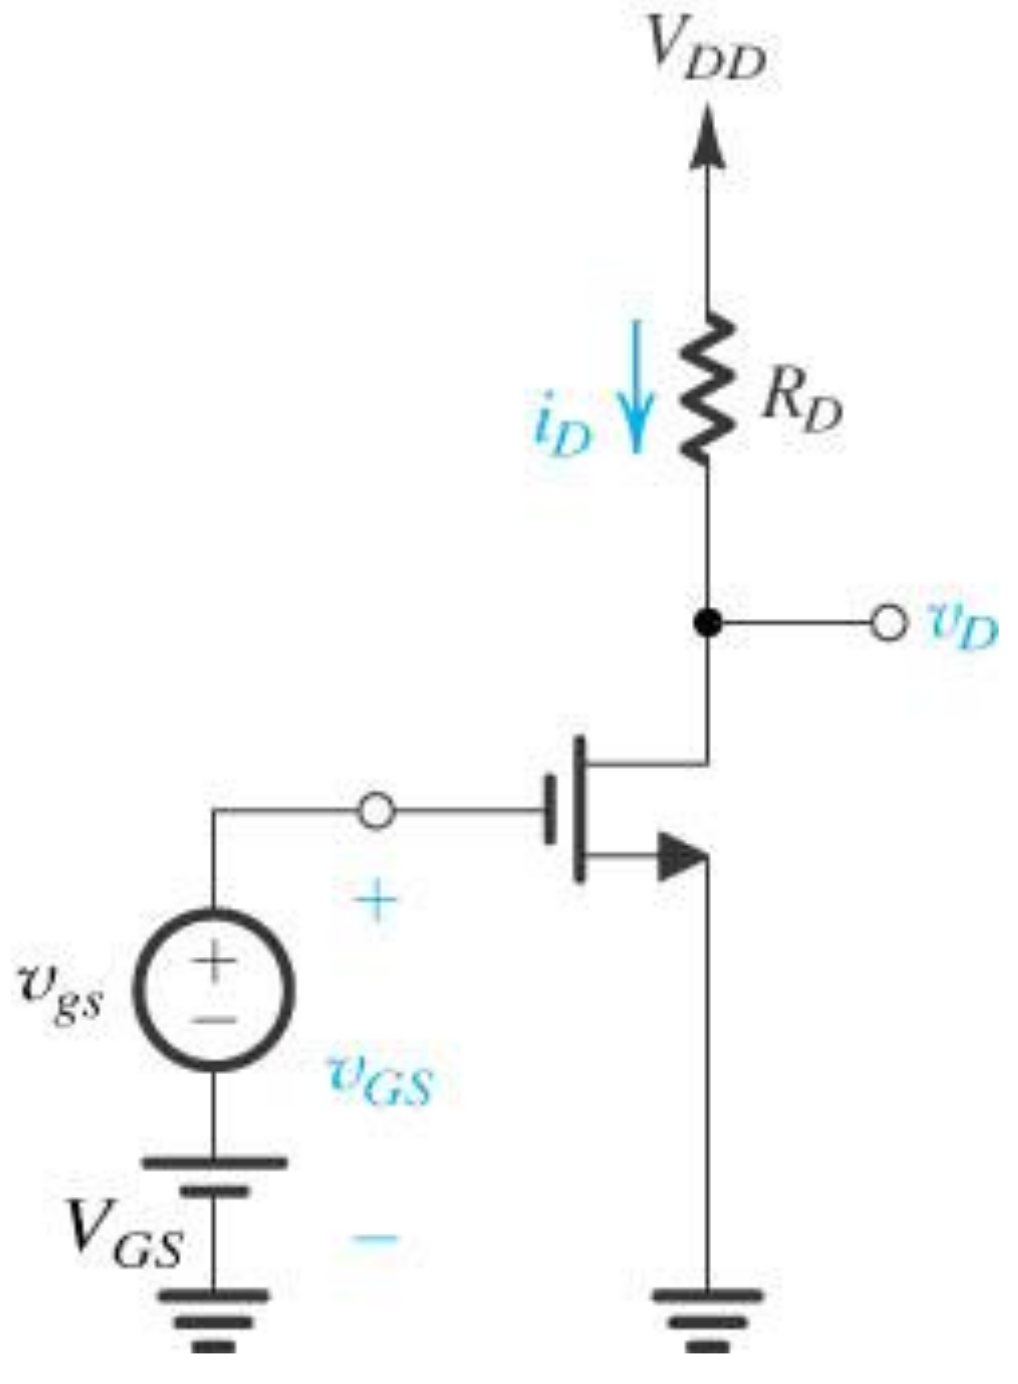
\includegraphics[width=0.25\textwidth]{imagens/1.png}
  \label{fig:1}
\end{figure}
 
\question[2] Usando o teorema de Miller, estime a capacitância de entrada e a capacitância de saída do circuito da Figura. Use $\lambda > 0$ (inclusive para a fonte de corrente) e desconsidere qualquer outra capacitância.

\begin{figure}[!h]
  \centering
  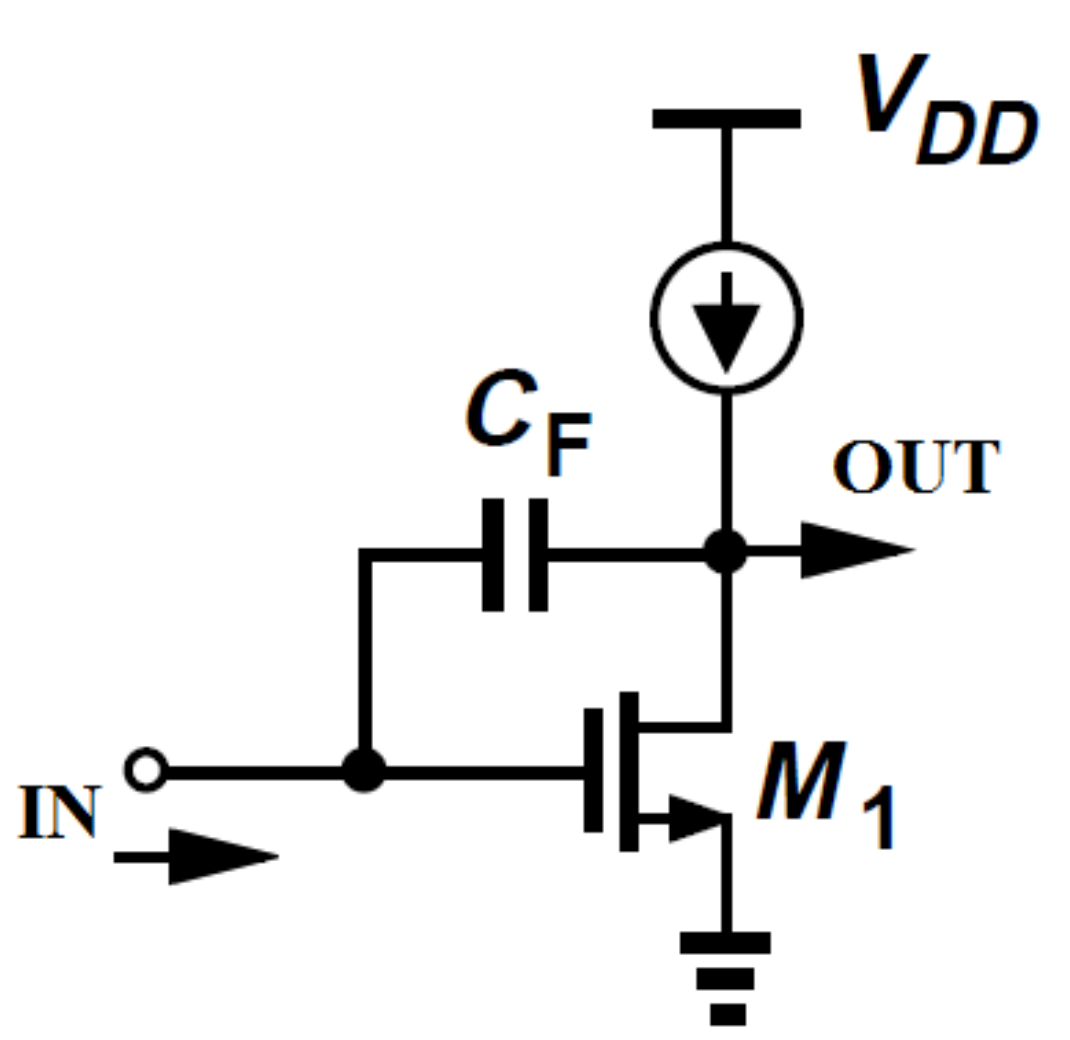
\includegraphics[width=0.25\textwidth]{imagens/2.png}
  \label{fig:2}
\end{figure}

\question[2] Explique e demonstre matematicamente porque o amplificador porta comum e dreno comum são conhecidos como seguidor de corrente e seguidor de tensão, respectivamente.

\question Para o amplificador porta comum da Figura:

\begin{parts}
 \part[1] Apresente o modelo de pequenos sinais;
 \part[1] Determine a função de transferência;
 \part[1] Encontre as constantes de tempo;
 \part[1] Faça um rascunho do módulo da resposta em frequência do amplificador (gráfico).
 \label{item:e}
 \part[1] No gráfico do item \ref{item:e} indique as frequências de corte, aproximadamente.
\end{parts}

\hspace{5.5mm}

Considere:

\hspace{10mm}

\begin{minipage}[m]{0.3\textwidth}
\begin{itemize}
    \item $\lambda = 0$;
    \item $R_D = 10$ $k\Omega$
    \item $R_S = 5$ $k\Omega$
    \item $C_{IN} = 25 pF$
    \item $C_{L} = 80 pF$
    \item $W/L = 60$
    \item $k'_n = 100$ $\mu A/V^2$
    \item $V_{OV} = 0,8$ V
\end{itemize}
\end{minipage}
\hspace{5mm}
\begin{minipage}[m]{0.4\textwidth}
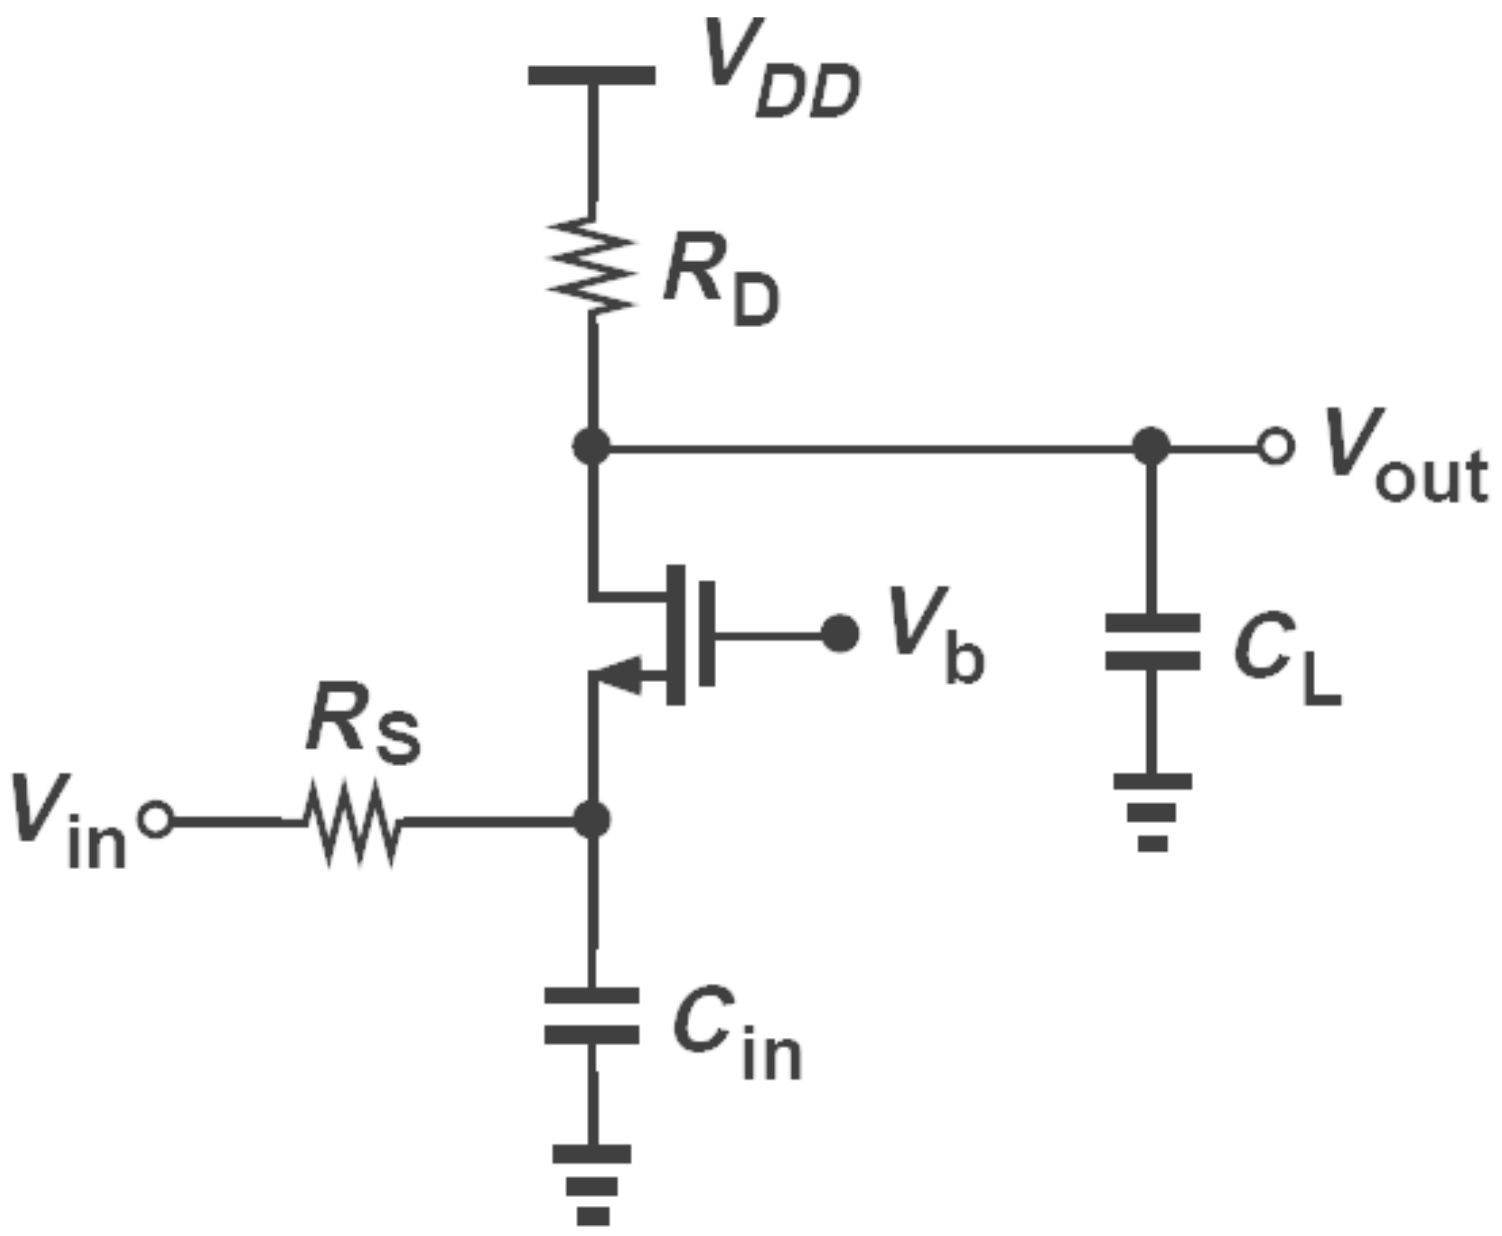
\includegraphics[width=\textwidth]{imagens/3.png}
\end{minipage}












\end{questions}

\end{document}
